\documentclass{beamer}
\usepackage[utf8]{inputenc}
\usepackage{graphicx}
\usepackage[ngerman]{babel}
\usepackage[T1]{fontenc}
\usepackage{verbatim}

\author{Marlene Knoche}
\title{\LaTeX-Seminar}
\begin{document}

\begin{frame}

\maketitle

\end{frame}

\begin{frame}

\tableofcontents

\end{frame}

\section{Was ist \LaTeX?}

\begin{frame}
\centering
\huge{Was ist \LaTeX?}
\end{frame}

\begin{frame}{Geschichte - I}
\begin{itemize}
\item Ursprünglich wurde \TeX\; von Donald E. Knuth entwickelt
\item \LaTeX\; ist Sammlung von \TeX-Makros von Leslie Lamport 
\end{itemize}

\begin{figure}
\centering
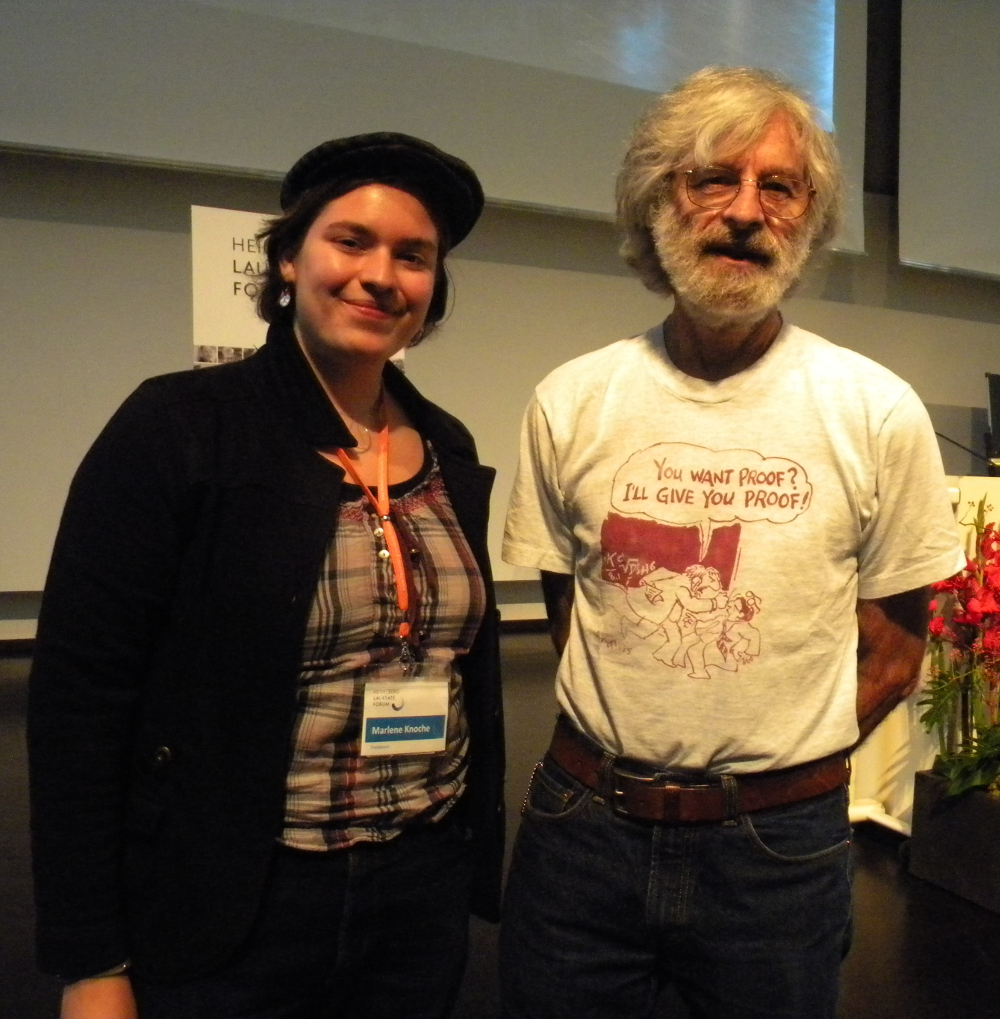
\includegraphics[scale=0.5]{pics/leslielamport.jpg}
\caption{Leslie Lamport und ich in Heidelberg beim HLF14 2014}
\end{figure}
\end{frame}

\begin{frame}{Geschichte - II}
\begin{itemize}
\item Entwicklung 1990 von Lamport eingestellt
\item Seit 1989 ist \LaTeX $2_{\varepsilon}\;$ von Frank Mittelbach, Chris Rowley und Rainer Schöpf weiter entwickelt worden
\item Seit Mitte der 1990er ist \LaTeX $2_{\varepsilon}\;$ am weitesten verbreitete Methode, \TeX\; zu nutzen
\end{itemize}
\end{frame}

\begin{frame}{WYSIWYG vs WYGIWYM}

\begin{block}{WYSIWYG}
= \textbf{W}hat \textbf{y}ou \textbf{s}ee \textbf{i}s \textbf{w}hat \textbf{y}ou \textbf{g}et

Formatierung wird direkt angezeigt
\end{block}

\begin{block}{WYGIWYM}
= \textbf{W}hat \textbf{y}ou \textbf{g}et \textbf{i}s \textbf{w}hat \textbf{y}ou \textbf{m}ean

Formatierung wird beschrieben
\end{block}

\begin{itemize}
\item \LaTeX \; ist Vertreter für WYGIWYM
\end{itemize}
\end{frame}

\begin{frame}{Betriebssysteme und Editoren}

\begin{itemize}
\item Editoren und \LaTeX-Umgebung für alle Plattformen verfügbar
\item TeXworks standardmäßig bei Installation dabei (alle Plattformen)
\item Andere Editoren: 
	\begin{itemize}
	\item TeXlipse Plugin für Eclipse (alle Plattformen)
	\item Texmaker (alle Plattformen
	\item TeXstudio (alle Plattformen)
	\item Kile (KDE(Linux), Windows)
	\item TeXnicCenter (Windows)
	\item \ldots
	\end{itemize}
\end{itemize}

\end{frame}

\section{Grundlegendes}
\begin{frame}
\centering
\huge{Grundlegendes}
\end{frame}


\begin{frame}[fragile]{Syntax}

\begin{itemize}
\item Groß- und Kleinschreibung ist relevant!
\item Kommentare beginnen mit \%-Zeichen.
\end{itemize}

\begin{block}{Befehle:}

\begin{itemize}
\item $\backslash$\texttt{Befehlsname}
\item $\backslash$\texttt{Befehlsname}\{\texttt{Option}\}
\item $\backslash$\texttt{Befehlsname}[\texttt{Option}]\{\texttt{Option}\}
\end{itemize}
\end{block}

\begin{block}{Umgebungen:}
\begin{verbatim}
	\begin{Umgebungsname}
	Text und/oder Befehle
	\end{Umgebungsname}
\end{verbatim}

Umgebungen müssen immer geschlossen werden.

Zusätzliche Optionsplatzhalter sind möglich.

\end{block}


\end{frame}

\begin{frame}[fragile]{Grundstruktur Dokument}
\begin{enumerate}
\item Definition einer Dokumentenklasse
	\begin{itemize}
		\item \begin{verbatim}\documentclass[Option]{Dokumentenklasse}\end{verbatim}
		\item z.B. article (scrartcl in KOMA-Script), report (srcreprt in KOMA-Script)
	\end{itemize}
\item Packages nachladen und Konfiguration des Dokumentes
	\begin{itemize}
		\item Packages laden: \begin{verbatim}\usepackage[Option]{Packagename}\end{verbatim}
		\item Angabe von Meta-Informationen wie Autor oder Titel
	\end{itemize}
\item Dokumenteninhalt innerhalb der \texttt{document}-Umgebung
	\begin{itemize}
	\item \begin{verbatim} \begin{document} Text und Befehle \end{document}
	\end{verbatim}
	\end{itemize}
\end{enumerate}
\end{frame}

\begin{frame}[fragile]{Minimalbeispiel}

Minimalistisches Beispiel ohne Packages.

\begin{verbatim}
	\documentclass{article}
	\begin{document}
	\section{Hallo Welt!}
	Ich bin der tolle Text auf der ersten Seite!
	\end{document}
\end{verbatim}
\end{frame}

\section{Dokument}
\begin{frame}
\centering
\huge{Dokument}
\end{frame}

\begin{frame}[fragile]{Gliederungsebenen}
\begin{itemize}
\item Mögliche Gliederungsebenen abhängig von verwendeter Dokumentenklasse
\item section, subsection und subsubsection in allen Dokumentenklassen verfügbar
\item weitere Ebenen: part, chapter (der section übergeordnet, Dokumentenklasse report), paragraph und subparagraph (der subsubsection zugeordnet)
\item Syntax jeweils \begin{verbatim} \gliederungsebene{Name} \end{verbatim}
\item Beispiel siehe Minimalbeispiel
\end{itemize}
\end{frame}

\begin{frame}[fragile]{Text formatieren}
\begin{itemize}
\item \textbf{fett}: \begin{verbatim}\textbf{fett}\end{verbatim}
\item \textit{kursiv}:\begin{verbatim}\textit{kursiv}\end{verbatim}
\item \texttt{Schreibmaschine}: \begin{verbatim}\texttt{Schreibmaschine}\end{verbatim}
\item {\rmfamily \scshape Kapitälchen}: \begin{verbatim}\textsc{Kapitälchen}\end{verbatim}
\end{itemize}
\end{frame}

\begin{frame}[fragile]{Aufzählungen/Listen - I}
\begin{itemize}
\item drei Arten von Aufzählungen: \texttt{itemize} (Stichpunkte), \texttt{enumerate} (Nummerierung), \texttt{description} (Beschreibungen)
\item lassen sich Kombinieren und beliebig verschachteln
\item Syntax: \begin{verbatim} \begin{listenart} \item Inhalt \end{listenart} \end{verbatim}
\end{itemize}
\end{frame}

\begin{frame}[fragile]{Aufzählungen/Listen - III (Beispiel Itemize)}

\begin{minipage}{0.4\textwidth}
\begin{verbatim}
	\begin{itemize}
	\item Stichpunkt 1
	\item[] 42
	\item Neuer Stichpunkt
	\end{itemize}
\end{verbatim}
\end{minipage}
\begin{minipage}{0.4\textwidth}

	\begin{itemize}
	\item Stichpunkt 1
	\item[] 42
	\item Neuer Stichpunkt
	\end{itemize}

\end{minipage}


\end{frame}

\begin{frame}[fragile]{Aufzählungen/Listen - IV (Beispiel Enumerate)}

\begin{minipage}{0.4\textwidth}
\begin{verbatim}
	\begin{enumerate}
	\item Stichpunkt 1
	\item [] 42
	\item Neuer Stichpunkt
	\end{enumerate}
\end{verbatim}
\end{minipage}
\begin{minipage}{0.4\textwidth}

	\begin{enumerate}
	\item Stichpunkt 1
	\item [] 42
	\item Neuer Stichpunkt
	\end{enumerate}

\end{minipage}

\end{frame}

\begin{frame}[fragile]{Aufzählungen/Listen - V (beispiel Description)}

\begin{minipage}{0.4\textwidth}
\begin{verbatim}
	\begin{description}
	\item [Text] Stichpunkt 1
	\item [Ultimativ] 42
	\item [Neuer] Stichpunkt
	\end{description}
\end{verbatim}
\end{minipage}
\begin{minipage}{0.5\textwidth}

	\begin{description}
	\item [Text] Stichpunkt 1
	\item [Ultimativ] 42
	\item [Neuer] Stichpunkt
	\end{description}

\end{minipage}

\end{frame}

\begin{frame}{Grafiken}
\end{frame}

\begin{frame}{Tabellen}
\end{frame}

\begin{frame}{Formeln}
\end{frame}

\begin{frame}{Quellcode einbinden}
\end{frame}

\begin{frame}{Fußnoten}
\end{frame}

\begin{frame}{Dokument formatieren - I}
Titelseite basics
Schriftgröße
Seitenlayout
\end{frame}

\begin{frame}{Dokument formatieren - II}
Labels und Referenzen
Verzeichnisse einbinden
Numerierung der Seiten
\end{frame}


\section{Weiterführendes}
\begin{frame}
\centering
\huge{Weiterführendes}
\end{frame}

\begin{frame}{Aufteilen von Dokumenten}
input vs include
\end{frame}


\section{Mein Template}
\begin{frame}
\centering
\huge{Mein Template}
\end{frame}

\section{Ressourcen}
\begin{frame}
\centering
\huge{Ressourcen}
\end{frame}

\begin{frame}{Literatur und Links}
\begin{description}
\item[LaTeX kurz und gut] O'Reilly Verlag, 3. Auflage, Matthias Kalle Dalheimer und Karsten Günther, \\
ISBN: 978-3-89721-542-9
\item[TEX Stackexchange] \url{http://tex.stackexchange.com}
\item[Mein GitHub-Account] \url{https://github.com/Sanguinik}
\item[Mein Blog] \url{http://www.sanguinik.de}
\end{description}
\end{frame}

\begin{frame}
\begin{center}
\huge{Fragen?}
\end{center}
\end{frame}

\end{document}